% CHAPTER
\chapter{Preliminary discussion}
\label{chap:prelim}

In this chapter, we review the equioscillation property of best approximations and discuss composite approximations $f_{k+1}=g(f_k)$ used for computing the sign and square root functions. In particular, we introduce the \textit{Newton-Schulz} iteration for approximating $\sgn(x)$, for which the iteration function $g$ is a polynomial. These ideas will be important in later chapters, as we will construct scaled composite approximations $f_{k+1}=g_{k+1}(f_k)$, assessing their quality by comparing them to the corresponding unscaled approximations, and checking whether or not they are best approximations by counting the number of equioscillation points in the error. Before we proceed, let us make the definitions of composite polynomials and degrees of freedom precise.

\section{Composite polynomials and degrees of freedom}

%\section{Motivation: matrix decompositions}

%For a Hermitian matrix $A \in \C^{n\times n}$, there exists an eigendecomposition $A=ZDZ^{-1}$ where $D=\text{diag}(\lambda_1,\dots,\lambda_n)$ is a diagonal matrix comprising of a full set of $n$ eigenvalues of $A$. For a scalar function $f$ defined on the spectrum of $A$ (denoted $\Lambda(A)$), we define 
%\[f(A):= Z f(D) Z^{-1} = Z \text{diag}(f(\lambda_1),\dots,f(\lambda_n))Z^{-1}.\]
%A matrix function of this form is referred to as a \textit{primary matrix function}. We consider the matrix equation $f(A)=X$ for some $X \in \C^{n\times n}$.  

%\bigskip{}

%As an example, $A$ is a square root of $X$ if $A^2=X$. It is clear from \cite[Theorem 1.29]{Higham} that an $X$ with no eigenvalues on the closed negative real axis has a unique square root $A$, which we refer to as the \textit{principal square root}. 

\begin{defn}\label{comppolydefn}
A bivariate polynomial $p(x,y)$ is said to be of degree $m$ if $p(x,x)$ is of degree $m$. A polynomial $p(x)$ is said to be \textit{$(k,m)$-composite} if
\begin{align}
    p(x) = p_k(x,p_{k-1}(x,p_{k-2}(\cdots(x,p_1(x,1))))) \label{poly}
\end{align}
for bivariate polynomials $p_i(x,y)$, $i=1,\dots,k$, each of degree $m$. We say that a $(k,m)$-composite polynomial is $pure$ if the $p_i(x,y)$ in \eqref{poly} are univariate, so that
\[p(x) = p_k(p_{k-1}(\cdots(p_1(x)))).\]
We will denote the space of pure $(k,m)$-composite polynomials by 
\[\Pee_{(k,m)}^{\text{comp}}=\{p_k \circ \cdots \circ p_1 : p_i \in \Pee_m\}.\]
Clearly $\Pee_{(k,m)}^{\text{comp}} \subset \Pee_{m^k}$, but equality doesn't hold: see \cite{rickards}. 
\end{defn}

The introduction of bivariate polynomials seems unnecessarily complicated, but is essential to allow the iteration function $g$ to depend on $x$ as well as the previous iterate\footnote{Dependence on $x$ was crucial for the square root iteration \eqref{funkyiter} in Chapter 1, for example.}. Many iterations we consider will take the form $f_{k+1}(x)=g(x,f_k(x))$.

\begin{defn}
The \textit{degrees of freedom} of a polynomial $p_n \in \Pee_n$ is the number of parameters required to completely determine $p_n$. We say that $p_n$ is a \textit{plain polynomial} if $p_n$ has $n+1$ degrees of freedom, that is, $p_n(x) = \sum_{k=0}^n \alpha_k x^k$ where $\{\alpha_k\}_{k=0}^n$ is a set of independent, non-zero scalars.
\end{defn}

We observe that composing low-degree polynomials is an efficient way to generate polynomials of much higher degree, with respect to the degrees of freedom.

\begin{ex}
Consider two plain polynomials $p_m\in \Pee_m$, $p_n \in \Pee_n$. Then $p_m\circ p_n$ has degree $mn$, whilst having only $m+n+2$ degrees of freedom. Moreover, a polynomial $p \in \Pee_{(k,m)}^{\text{comp}}$ formed by composing $k$ plain polynomials of degree $m$ has degree $m^k$, yet only $k(m+1)$ degrees of freedom.
\end{ex}

%\section{Polynomial approximation}

%A fundamental result in mathematical analysis is the Weierstrass approximation theorem, which asserts that any continuous function $f$ on a closed, bounded interval $I$ can be uniformly approximated by a polynomial to any given accuracy; in particular we can find a sequence $p_n \in \Pee_n$ such that $\norm{f-p_n}_{\infty,I}\to 0$ as $n\to\infty$. A natural question to ask is how quickly these polynommial approximants converge as $n\to\infty$. We briefly discuss  methods of polynomial approximation and their level of optimality.

%\subsection{Truncation}

%Lebesgue's 1898 proof of the Weierstrass approximation theorem \cite{Leb} exploits the fact that a polygonal curve (a function of the form $g(x)=Ax+B+\sum_{i=1}^k C_i |x-x_i|$) can be chosen to uniformly approximate $f$. This reduces the problem to uniformly approximating $|x|$ with polynomials, which can be achieved (after rescaling the function to the interval $[-1,1]$) by truncating the Taylor series\footnote{The series is indeed convergent for $x \in [-1,1]$: applying Stirling's formula shows that the coefficients of \eqref{1} are $O(k^{-3/2})$, hence the series is $O(k^{-1/2})$, thus convergent.}
%\begin{align}
%    |x| = \sqrt{1+(x^2-1)} = \sum_{k=0}^\infty \binom{1/2}{k} (x^2-1)^k. \label{1}
%\end{align}
%Truncating Taylor series expansions is one way to obtain polynomial approximants for smooth functions. Whilst convenient for more theoretical work, truncating in this way can be far from optimal, as the following example demonstrates (inspired by \cite[Exercise 10.9]{ATAP}). 

%\begin{ex} \label{chebtrunc}
%Let $f(x)=e^x$ on $[-1,1]$ and $F_n(x) = \sum_{k=0}^n x^k/k!$ be its Taylor series truncation. Clearly $\norm{f-F_n}_\infty = O(1/(n+1)!)$ as $n\to\infty$, but we can obtain a much smaller error by considering truncations $f_n$ of the Chebyshev series $f(x) = \sum_{k=0}^\infty a_k T_k(x)$, where 
%\begin{align}
%    a_k = \dfrac{2}{\pi} \int_{-1}^1 \dfrac{f(x)T_k(x)}{\sqrt{1-x^2}}\,dx \qquad (k \geq 1), \label{chebcoeff}
%\end{align}
%and $a_0$ is given by $1/2$ the value of \eqref{chebcoeff}. Substituting $x=\cos\theta$ gives the formula
%\[a_k = \dfrac{2}{\pi}\int_0^\pi f(\cos\theta)\cos(k\theta)\, d\theta,\]
%and similar for $a_0$, so we obtain $a_k = 2I_k(1)$ for $k\geq 1$ and $a_0=I_0(1)$, where $I_k$ is the \textit{modified Bessel function of the first kind}
%\[I_k(z)= \dfrac{1}{\pi}\int_0^\pi e^{z\cos\theta}\cos(k\theta)\,d\theta.\]
%The $a_k$ decay much faster than $1/k!$, which can be seen by applying the estimate
%\[e^{-z} < \Gamma(\nu+1)\left(\dfrac{2}{z}\right)^\nu e^{-z}I_\nu(z) < \dfrac{1}{2}(1+e^{-2z}), \qquad z>0, \quad \nu >-1/2,\]
%proved by Luke in 1972 \cite[p. 63]{Luke}. Setting $z=1$ and $\nu=k$, we find that
%\[\dfrac{1}{2^k k!}<I_k(1)< \dfrac{e}{2^k k!},\]
%hence $a_k = O(1/(2^k k!))$. Then, by \cite[Theorem 4.1]{ATAP}, we know that
%\[f(x)-f_n(x) = \sum_{k=n+1}^\infty a_k(T_k(x)-T_{m_k}(x)),\]
%where $m_k=|(k+n-1)\,\text{mod}\, 2n -(n-1)|$ is the aliased value of $k$. Therefore
%\[|f(x)-f_n(x)| \leq 2 \sum_{k=n+1}^\infty |a_k|=O\left(1/(2^n(n+1)!)\right).\]

%\subsection{Interpolation}

%A degree $n$ polynomial approximant to $f$ can also be generated by interpolating through $n+1$ points on the interval. The choice of grid (i.e$.$ the set of interpolation points) plays a major role in the error in the interpolant as $n\to\infty$. In fact, if $p_n \in \Pee_n([-1,1])$ is the (unique) interpolant to $f$ of degree $n$ and $\Lambda_n$ is the Lebesgue constant, i.e$.$ the operator norm of the bounded linear operator 
%\[C([-1,1]) \ni f \mapsto p_n \in \Pee_n,\]
%then one has (see e.g. \cite[Chapter 15]{ATAP})
%\[\Lambda_n \sim \dfrac{2^{n+1}}{ne\log n}, \qquad n\to\infty,\]
%if the grid is determined by equispaced points $x_j = -1 + 2j/n$, where $j=0,1,\dots,n$. This is in comparison to
%\[\Lambda_n \sim \dfrac{2}{\pi}\log n, \qquad n\to\infty,\]
%if the grid is determined by the Chebyshev points $x_j = \cos (j\pi/n)$. These asymptotic approximation demonstrate that, given the worst possible data, interpolation in equispaced points is not a good idea: Lebesgue constants for such grids grow faster than any polynomial, whereas Lebesgue constants for Chebyshev grids grow slower than any polynomial. In fact, for any grid we have the inequality
%\[\Lambda_n \geq \dfrac{2}{\pi}\log(n+1)+\dfrac{2}{\pi}\left(\gamma+\log\dfrac{4}{\pi}\right),\]
%where $\gamma\approx 0.577$ is Euler's constant \cite{?}, so we observe that Chebyshev grids come close to minimising the value of the Lebesgue constant.

%\bigskip{}

%Our observations are further backed up by the landmark results of Runge and Bernstein, who respectively said that for equispaced grids, there is an analytic function $f$ such that $p_n \not\to f$ \cite{?}, but for Chebyshev grids, $p_n \to f$ provided that $f$ is Lipschitz \cite{?}.

\section{Best approximation and equioscillation}

To analyse how well a polynomial $p \in \Pee_n$ is approximating a function $f \in C(I)$, where $I$ is a closed, bounded interval, we can consider for $p_n \in \Pee_n$ the error
\begin{align}
    \norm{(f-p_n)w}_{\infty,I}, \label{error}
\end{align}
where $w \in C(I)$ is a positive \textit{weight function}. In the best-case scenario, $p$ will minimise \eqref{error} over all $p_n \in \Pee_n$. Such an approximation is known as the \textit{best approximation}, or \textit{minimax}, to $f$ with respect to $w$. Common weights include $w(x) \equiv 1$ (corresponding to the uniform error) and $w(x)=1/f(x)$ (corresponding to the relative error, assuming that $f(x)> 0$ on $I$). The best approximation exhibits a remarkable equioscillation property, as seen in e.g$.$ \cite[Chapter II]{AkhApprox}. 

%In \cite{stahl2003}, Stahl proves that for $\alpha>0$, the best rational approximant to $|x|^\alpha$ on $[-1,1]$ in the uniform sense satisfies 
%\[E_{n,n} \sim 2^{2+\alpha}\left|\sin\left(\dfrac{\pi\alpha}{2}\right)\right|\exp(-\pi\sqrt{\alpha n}), \qquad n\to\infty.\]

\begin{defn}
A function $f \in C(I)$ on a closed, bounded interval $I$ \textit{equioscillates} between $k$ extreme points if there exist $\{x_i\}_{i=1}^k \subset I$ such that $x_1 < x_2 < \cdots < x_k$ and for some $j \in \{0,1\}$,
\[f(x_i) = (-1)^{i+j}\norm{f}_{\infty,I}, \qquad i=1,\dots,k.\]
\end{defn}

\begin{thm}[Equioscillation Theorem]\label{equioscthm}
Let $f\in C(I)$ be a real function on a closed, bounded interval $I$. For every $n \in \N$ and weight function $w \in C(I)$, there is a unique best approximation $p^* \in \Pee_n$ to $f$ with respect to $w$. Moreover, if $p \in \Pee_n$, then $p = p^*$ if and only if $(f-p)w$ equioscillates between at least $n+2$ extrema.
\end{thm}

\begin{figure}[t!]
    \centering
    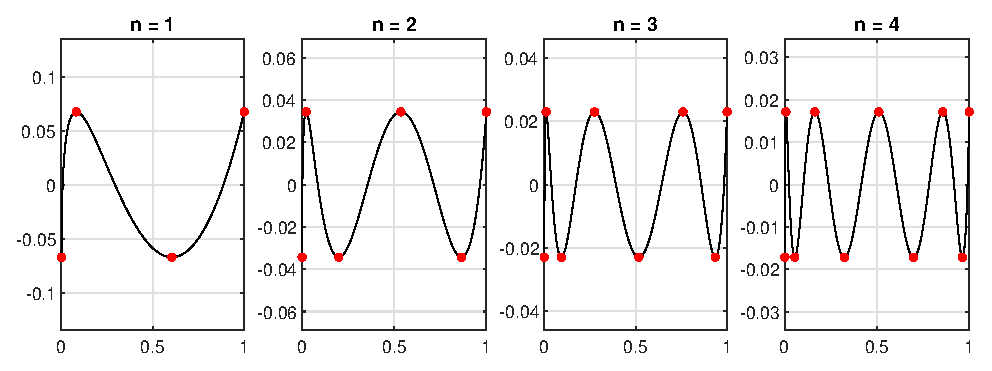
\includegraphics[width=\textwidth,height=\textheight,keepaspectratio]{figures/chapter_2/sqrtnew.eps}
    \caption{The equioscillation property demonstrated: error $E_{2n}(x)=\sqrt{x}-p^*_{2n}(x)$ in the uniform best approximations $p^*_{2n}\in\Pee_{2n}$ to $\sqrt x$ on $[0,1]$.}
    \label{fig:sqrt}
\end{figure}

In \cite[Lemma 2]{YujiZolotFreund}, Nakatsukasa and Freund provide an equioscillation result for \textit{rational} best approximations on a disjoint union of closed, bounded intervals in the uniform sense. In Theorem \ref{disjointrat}, we will generalise and prove their result to include errors equipped with a positive weight function, allowing for the same result in the relative sense, for example. We highlight the result in the case of polynomials, since it will be crucial in our construction of a composite polynomial approximation to the sign function in the next chapter.

\begin{corollary}\label{disjoint}
Suppose that $f\in C(I\cup J)$ is a real function on disjoint, closed, bounded intervals $I,J$. Then $p \in \Pee_n$ is the unique best approximation to $f$ with respect to $w$ if $(f-p)w$ equioscillates between at least $n+3$ extrema.
\end{corollary}

%\begin{proof}
%By contradiction. If $(f-r)w$ equioscillates between $n+3$ extrema %$\{x_i\}_{i=1}^{n+3}$ but there exists $p' \in \Pee_n$ such that 
%\[\norm{(f-p')w}_{\infty,I\cup J} < \norm{(f-p)w}_{\infty,I\cup J},\]
%then $(p-p')w$ takes alternating signs at the $x_i$, hence $(p-p')w$ vanishes at a minimum of $n+1$ points (this would be $n+2$ if we were not considering a disjoint union). Since $w>0$ and $p-p' \in \Pee_n$, we must have $p-p'=0$, a contradiction.
%\end{proof}

One final result on best approximations, mentioned briefly in \cite[p. 2]{Erem} as a remark, is the following. We present it as a lemma with a full proof.

\begin{lemma}\label{symm}
Let $n\in\N$, and suppose $f\in C(I)$ is an odd function on an interval $I$ symmetric about the origin. Then the best uniform approximation $p^* \in \Pee_{2n}$ is an odd function. Hence $p^*(x)=xh(x^2)$ for some $h \in \Pee_{n-1}$.
\end{lemma}

\begin{proof}
Define $q(x)=(p^*(x)-p^*(-x))/2$. Then $q(-x)=-q(-x)$, so $q$ is odd. As a result, if we write $q(x)=\sum_{k=0}^{2n} \alpha_k x^k$ for some $\alpha_k \in \R$ and compare the coefficients of the equation $q(x)=-q(-x)$, we find that $\alpha_i=0$ for $i=0,2,\dots,2n$. Hence $q(x)=\sum_{k=0}^{n-1} \alpha_{2k+1}x^{2k+1}$, so we can write $q(x)=xh(x^2)$ where 
\[h(x)=\sum_{k=0}^{n-1}\alpha_{2k+1}x^k \in \Pee_{n-1}.\]
We show that $p^*=q$. To see this, we use that $f$ is an odd function and $I$ is symmetric about the origin, so that $x \in I$ if and only if $-x \in I$, to obtain
\[ |q(x)-f(x)| = \left|\dfrac{p^*(x)-f(x)}{2}-\dfrac{p^*(-x)-f(-x)}{2}\right| \leq \norm{p^*-f}_{\infty,I},\]
by the triangle inequality. Hence $\norm{q-f}_{\infty,I} \leq \norm{p-f}_{\infty,I}$ for all $p\in\Pee_{2n}$. By uniqueness of the best approximation, we must have $p^*=q$.
\end{proof}

\textit{Remark.} In the context of Lemma \ref{symm}, the maximum uniform error of $p^*$ on $I^+=\{x \in I: x \geq 0\}$ will be identical to that on $I^-=\{x \in I: x \leq 0\}$ by symmetry, so the problem of finding the best approximation $p^*\in \Pee_{2n}$ to $f$ on $I$ is equivalent to finding the best odd approximation on $f|_{I^+}$, and such an approximation will be characterised by $f-p^*$ having at least $n+1$ equioscillation points in $I^+$. 

\subsection{Rational best approximation and equioscillation}

We occasionally discuss rational functions in this dissertation, and use the results of composite rational functions\footnote{Analogous to Definition \ref{comppolydefn}, a composite rational function is defined using bivariate rational functions, which we include in Appendix \ref{compratappendix}. This is the same definition as used in \cite{Yuji}.} as motivation for considering similar composite polynomial approximations. As such, we shall briefly discuss the analogues of this section for rational functions. 

\bigskip{}

Suppose we approximate a continuous function $f\in C(I)$ with a rational function $r_{m,n} \in \Arr_{m,n}(I)$. A \textit{rational best approximation} to $f$ with respect to a positive weight function $w$ minimises an error of the form
\[\norm{(f-r)w}_{\infty,I}\]
over all $r\in \Arr_{m,n}(I)$. A characterisation of the best approximations in terms of an equioscillating error curve also exists for rational functions \cite[Chapter II]{AkhApprox}.

\begin{thm}[Equioscillation theorem for rational functions]\label{equithmrats}
Let $f \in C(I)$ be a real function on a closed, bounded interval $I$. For every $m,n \in \N$ and weight function $w\in C(I)$, there is a unique rational best approximation $r^* \in \Arr_{m,n}$ to $f$ with respect to $w$. Moreover, if $r=P/Q$ for $P \in \Pee_m$, $Q \in \Pee_n$, then $r = r^*$ if and only if $(f-r)w$ equioscillates between at least $m+n+2-d_r$ extrema, where 
\[d_r=\min\{m-\deg P,n-\deg Q\}\]
is the \emph{defect} of $r$.
\end{thm}

Finally, we include the equioscillation result of Nakatsukasa and Freund, which we have generalised to include a weight function. This will later be used to verify the optimality of rational approximations to the sign function.

\begin{thm}\label{disjointrat}
Let $m,n \in \N$, $r \in \Arr_{m,n}$ and $f \in C(I \cup J)$, where $I,J$ are disjoint closed, bounded intervals. If $(f-r)w$ equioscillates between at least $m+n+3$ extrema, then $r$ is the (unique) rational best approximation to $f$ in $\Arr_{m,n}$ with respect to $w$.
\end{thm}

\begin{proof}
By contradiction. If $(f-r)w$ equioscillates between $m+n+3$ extrema $\{x_i\}_{i=1}^{m+n+3}$ but there exists $r' \in \Arr_{m,n}$ such that 
\[\norm{(f-r')w}_{\infty,I\cup J} < \norm{(f-r)w}_{\infty,I\cup J},\]
then $(r-r')w$ alternates in sign at the $x_i$, hence $(r-r')w$ vanishes at a minimum of $m+n+1$ points (this would be $m+n+2$ points if we were not considering a disjoint union). Since $w>0$ and $r-r' \in \Arr_{m+n,2n}$, we must have $r-r'=0$, a contradiction.
\end{proof}

\section{Matrix iterations and Newton's Method}

In the introduction, we saw how matrix iterations can be interpreted as composite polynomial or rational approximations to a matrix function $f(A)$ in terms of the initial guess $X_0$ (usually $X_0=A$). When deriving matrix iterations, it is common to first apply Newton's Method to an algebraic equation which has $f(A)$ as a solution, then choose an initial guess $X_0$ that accelerates the algorithm. Recall Newton's Method for finding a root $x^*$ of $f(x)=0$, where $f$ is a differentiable scalar function: for an initial guess $x_0$, we define the sequence
\begin{align}
    x_{k+1}=g(x_k):=x_k - \dfrac{f(x_k)}{f'(x_k)}, \qquad k=0,1,2,\dots,\label{NMeth}
\end{align}
provided that $f'(x_k)\neq 0$ for all $k$. Newton's Method converges if $x_0$ is sufficiently close to $x^*$, in this case converging quadratically \cite[Theorem 1.8]{Suli}. Due to the division by $f'(x_k)$ in \eqref{NMeth}, we often find that scalar Newton iterations contain inverses of the previous iterate. This is unfavourable if the underlying iteration function $g$ is then used to derive matrix iterations $X_{k+1}=g(X_k)$, since each iteration requires a new inverse to be computed, such as in the Newton iteration for the matrix square root \eqref{newty}.

\bigskip{}

The following example demonstrates this pitfall, and shows how considering a different algebraic equation can result in a sequence that doesn't require a new inverse to be computed at each iteration.

\begin{ex}\label{altexample}
To obtain an approximation to $\sqrt{x}$ on some interval $I$, we can fix $\lambda \in I$ and apply Newton's Method to functions for which $\sqrt{\lambda}$ is a solution. This generates iterates $x_k(\lambda)\approx \sqrt{\lambda}$ which can then be generalised to a function over the whole interval by defining $f_k(\lambda):=x_k(\lambda)$. Applying Newton's Method to the equation $f(x)=x^2-\lambda$, we obtain the iteration
\begin{align}
    f_{k+1}(x) = \dfrac{1}{2}\left(f_k(x) + \dfrac{x}{f_k(x)}\right)=:g(x,f_k(x)), \label{iter}
\end{align}
which is the scalar Newton iteration seen in \eqref{funkyiter}. Alternatively, we could apply Newton's Method to $f(x)=1-\lambda/x^2$, which also has $\sqrt{\lambda}$ as a root. This gives
\begin{align}
    f_{k+1}(x) = \dfrac{f_k(x)}{2}\left(3 -\dfrac{f_k(x)^2}{x}\right)=:\tilde{g}(x,f_k(x)). \label{altnewt}
\end{align}
\end{ex}

\begin{figure}[t!]
\centering
   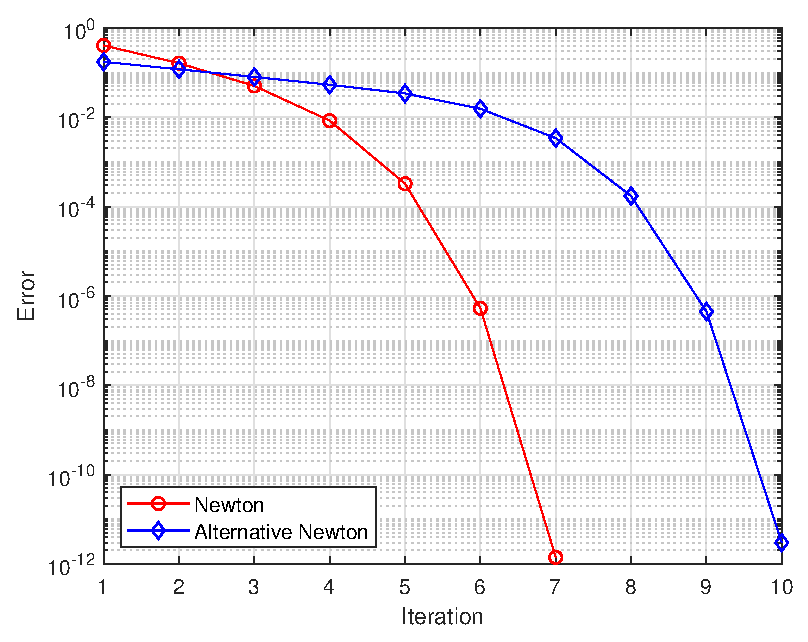
\includegraphics[width=0.7\textwidth,height=0.7\textheight,keepaspectratio]{figures/chapter_2/sqrt_newton_vs_alt.eps}
   \caption{Comparison of the maximum absolute uniform error in the standard Newton \eqref{funkyiter} and Alternative Newton \eqref{altnewt} iterates to $\sqrt{x}$ on $[\delta^2,1]$, where $\delta=0.1$.}
   \label{fig:sqrt_newt_vs_alt}
\end{figure}

\begin{rmk}
While the iteration function $\tilde{g}$ in \eqref{altnewt} is not a polynomial, the iterative process never divides by the previous iterate. Furthermore, it is clear that any initial guess $f_0$ that is a multiple of $x$ will produce polynomial approximations. We will refer to the iterations \eqref{altnewt}, with $f_0(x)=x$, as \textit{Alternative Newton} iterates. 
\end{rmk}

\newpage

Figure \ref{fig:sqrt_newt_vs_alt} compares the maximum uniform error in the Newton and Alternative Newton approximations to $\sqrt{x}$. Clearly, the alternative iterates underperform the standard iterates, which is to be expected since we are comparing the convergence of polynomial approximations to rational approximations. 

\subsection{Newton-Schulz iterations and the matrix sign function}

The conventional approach for removing inverses in matrix iterations of the form $X_{k+1}=g(X_k)$, where $g$ is a rational function, is to replace all instances of $X_k^{-1}$ with inversion-free approximations to them. This can be achieved by considering Newton's Method for the inverse of an invertible matrix $B$, given by
\begin{align}
    Y_{k+1}=Y_k(2I-BY_k), \label{schulzy}
\end{align}
as proposed by Schulz \cite{schulz}. Computing one step of Newton's Method for $X_k^{-1}$ by taking $Y_k = B = X_k$ in \eqref{schulzy}, we obtain the approximation $X_k^{-1} \approx X_k(2I-X_k^2)$. Newton iterations that approximate appearances of inverses in this way are referred to as \textit{Newton-Schulz} iterations. 

\bigskip{}

Let us find the Newton-Schulz iteration for the \textit{matrix sign function}. Analogous to the scalar sign function $\sgn(z)=z/\sqrt{z^2}$, where $\text{Re}(z)\neq 0$, we define\footnote{There are several equivalent definitions for matrix functions, which are discussed in detail in \cite[Chapter 1]{Higham}.} the sign of a matrix $A \in \C^{n\times n}$ with eigenvalues away from the imaginary axis by
\[\sgn(A)=A(A^2)^{-1/2},\]
where $B^{-1/2}$ denotes the inverse of the principal square root of $B$. In particular, this is well-defined since $A$ having no eigenvalues on the imaginary axis implies that $A^2$ has no eigenvalues on the closed negative real axis. In \cite[Section 1.3]{roberts}, Roberts shows that the iteration
\begin{align}
    X_{k+1}=\dfrac{1}{2}(X_k + X_k^{-1}), \qquad X_0 = A, \label{newtonsign}
\end{align}
converges to $\sgn(A)$. The iteration is precisely Newton's Method applied to the equation $X^2=I$, for which $\sgn(A)$ is clearly a solution, hence convergence is quadratic. Replacing $X_k^{-1}$ in \eqref{newtonsign} with the approximation $X_k(2I-X_k^2)$, we obtain the Newton-Schulz iteration
\begin{align*}
    X_{k+1}=\dfrac{X_k}{2}(3I - X_k^2), \qquad X_0 = A.
\end{align*}
This sequence also converges quadratically---provided that $\norm{I-A^2}_2<1$, where $\norm{\cdot}_2$ denotes the matrix 2-norm\footnote{It can be shown that the 2-norm of a matrix $B$ is equal to $\sigma_{\max}(B)$, the largest singular value of $B$. In the case of Hermitian matrices, the singular values are equal to the absolute values of the eigenvalues (see e.g$.$ \cite{NLAbook}), hence the Newton-Schulz iterates for $A$ are quadratically convergent when the eigenvalues of $A$ have magnitude strictly less than $\sqrt{2}$. It may thus be required to scale $A$ down to a matrix with suitably small eigenvalues before proceeding.}---though many iterations are required before quadratic convergence is seen \cite[Theorem 1.1]{chen}. Similarly, in the scalar case we could approximate $\sgn(x)$ using the functions
\begin{align}
f_{k+1}(x)=g(f_k(x)), \qquad g(x)=\dfrac{x}{2}(3-x^2),\label{scalarNSsign}
\end{align}

\begin{figure}[t!]
    \centering
    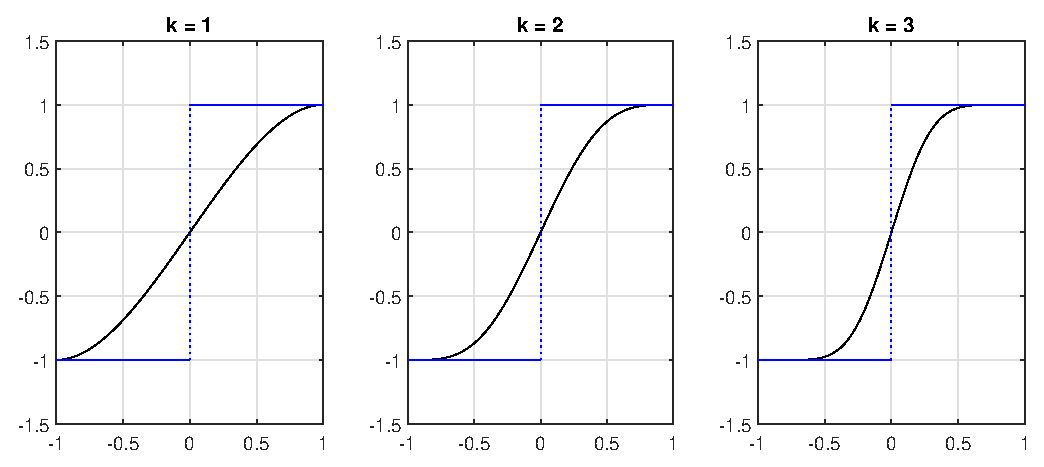
\includegraphics[width=\textwidth,height=\textheight,keepaspectratio]{figures/chapter_2/Sign_undershoot.eps}
    \caption{Newton-Schulz iterates $f_{k+1}(x)=f_k(x)(3-f_k(x)^2)/2$ (black) to $\sgn(x)$ (blue) on $[-1,1]$.}
    \label{fig:NSsigny}
\end{figure}

with $f_0(x)=x$. We shall refer to \eqref{scalarNSsign} as the \textit{(unscaled) Newton-Schulz} iteration for $\sgn(x)$. The first few iterations are illustrated in Figure \ref{fig:NSsigny}: the uniform error of the Newton-Schulz iteration is always 1 at the origin, so in practice we will consider the iteration on $X(\delta)=[-1,-\delta]\cup[\delta,1]$ for some $\delta \in(0,1)$. The maximum uniform error is then given by
\[\norm{f_k-\sgn}_{\infty,X(\delta)}=f_k(\delta).\]
\begin{rmk}
The Newton-Schulz iteration is one of a family of iterations of the form $X_{k+1}=g_{m,n}(X_k)$, where $g_{m,n}(x)=x p_m(1-x^2)/q_n(1-x^2)$, used for computing $\sgn(A)$. Here $p_m/q_n$ represents the $[m/n]$ \textit{Padé approximant} of $(1-x)^{-1/2}$ (see e.g. \cite[Section 3]{kenneylaubrational}). When $n=0$, we obtain composite polynomial approximations; in particular we recover the Newton-Schulz iteration for $(m,n)=(1,0)$. 
\end{rmk} 

%\subsection{Iterations for the square root function} 

%The result of Higham, Mackey, Mackey, and Tisseur states that, when $A^{1/2}$ is well-defined, any iteration $X_{k+1}=X_k h(X_k^2)$ converging to $\sgn\left(\begin{bsmallmatrix} 0 & A \\ I & 0 \end{bsmallmatrix}\right)$ gives rise to a coupled iteration 
%\[\begin{cases}Y_{k+1}=Y_k h(Z_k Y_k), & \quad Y_0 = A, \\ Z_{k+1} = h(Z_kY_k)Z_k, & \quad Z_0=I,\end{cases}\]
%in which $Y_k \to A^{1/2}$ and $Z_k \to A^{-1/2}$ as $k\to\infty$, with the same order of convergence as the $X_k$ \cite[Theorem 6.11]{Higham}. Taking $h(X)=(3I-X)/2$, the iteration function for the Newton-Schulz iterates to the sign function, we obtain
%\[\begin{cases}Y_{k+1}=Y_k (3I-Z_kY_k)/2, & \quad Y_0 = A, \\ Z_{k+1} = (3I-Z_kY_k)Z_k/2, & \quad Z_0=I,\end{cases}\]
%a coupled Newton-Schulz iteration for approximating the principal square root %$A^{1/2}$ and its inverse. Similarly we use the coupled scalar functions
%\begin{align}
%    \begin{cases}f_{k+1}(x)=f_k(x) (3-g_k(x)f_k(x))/2, & \quad f_0(x) = x, \\ g_{k+1}(x) = g_k(x)(3-g_k(x)f_k(x))/2, & \quad g_0(x)=1,\end{cases} \label{scalarNSsqrt}
%\end{align}
%to approximate $\sqrt{x}$ and $1/\sqrt{x}$ respectively. Figure \ref{fig:sqrterrors} sketches the error in the $f_k$ for the first 6 iterations.

%\begin{figure}[t!]
%    \centering
%    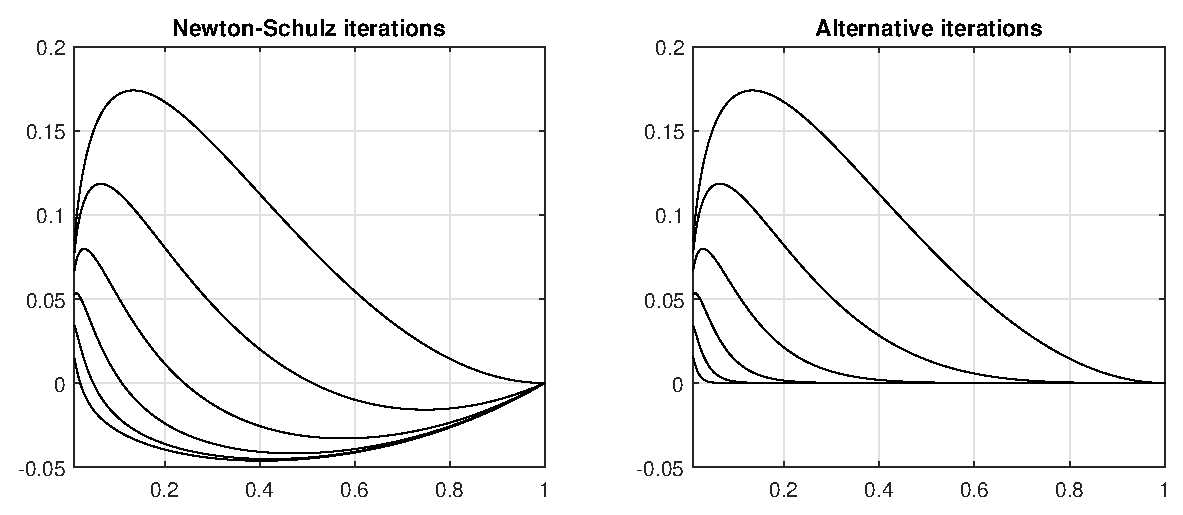
\includegraphics[width=\textwidth,height=\textheight,keepaspectratio]{sqrt_NSvsalt.eps}
%    \caption{Error $E_k(x)=\sqrt{x}-f_k(x)$ in the Newton-Schulz \eqref{scalarNSsqrt} and alternative \eqref{alt} iterations $f_k$ to $\sqrt{x}$ on $[0.1^2,1]$, for $k=1,\dots,6$.}
%    \label{fig:sqrterrors}
%\end{figure}





%One of the earliest methods of approximating the square root, \textit{Heron's Method}, dates back to the first century. For $\lambda>0$, Heron's Method for approximating $\sqrt{\lambda}$ is given by the following iterative process. Let $x_0$ be an initial guess. Then either $x_0$ or $\lambda/x_0$ is greater than $\sqrt{\lambda}$, whilst the other quantity is less than $\sqrt{\lambda}$. Let $x_1$ be the average of these two quantities. Repeat this averaging process with the new guess, and so forth. We can write this as $x_{k+1}=(x_k + \lambda x_k^{-1})/2$, where $k\in \N$. This process is equivalent to applying Newton's Method to solve the equation $x^2-\lambda=0$.

%Adopting the notation used in Appendix \ref{improvenewton}, the improved method is defined by $F_0(x)=C_0 f_0(x)$ and
%\begin{align}
%    F_{k+1}(x) = \dfrac{C_{k+1}}{2}\left(F_k(x)+\dfrac{x}{F_k(x)}\right),
%\end{align}
%where the constants $C_k$ are defined by
%\[C_0 = \dfrac{1}{\sqrt{s'_0 s''_0}}, \qquad C_k = %\dfrac{1}{\sqrt{N^*(S''_{k-1})}} \qquad (k\geq 1),\]
%and $S''_k=\max_{x\in I} F_k(x)/\sqrt x$.



%Alternatively we could approximate $\sqrt{\lambda}$ by first approximating $1/\sqrt{\lambda}$ with iterates $x_k$, then noting that $\sqrt{\lambda} \approx \lambda x_k$.

%\begin{ex}
%Suppose for $\lambda >0$ we want to approximate the value of $1/\sqrt{\lambda}$. This is equivalent to finding the positive root of $f(x)=x^2-1/\lambda=0$, so Newton's Method reads
%\[x_{k+1} = x_k - \dfrac{x_k^2-1/\lambda}{2x_k} = \dfrac{1}{2}\left(x_k +\dfrac{1}{\lambda x_k}\right).\]
%Alternatively, if we solved for the root of $f(x)=1/x^2-\lambda$, we obtain
%\begin{align}
 %   x_{k+1} = x_k - \dfrac{1/x_k^2-\lambda}{-2/x_k^3} = \dfrac{x_k}{2}\left(3 -\lambda x_k^2\right). \label{NEWTON2}
%\end{align}
%We similarly note that \eqref{NEWTON2} never divides by the previous iterate.
%\end{ex}


\subsection{Improved Newton's Method}\label{improvednewtonsection}

Despite being a quadratically converging sequence, the Newton-Schulz iteration \eqref{scalarNSsign} can take a large number of iterations to reach a suitably small error. For example, when $\delta=10^{-2}$, it takes 14 iterations to obtain an error $\ep<10^{-2}$ on $X(\delta)$. This is because the order of convergence is an \textit{asymptotic} property, and in practice, convergence breaks down into two phases:
\begin{itemize}
    \item the number of iterations required to reduce the error to some small value;
    \item the asymptotic behaviour given by the order of convergence.
\end{itemize}
Crucially, this means that we cannot guarantee that a quadratically convergent sequence (such as Newton's Method, or the Newton-Schulz iterates) will converge in a small number of iterations. 

\bigskip{}

Many contributions have been made to reduce the number of iterations required in the initial phase of convergence by considering scaled iterative processes, such as in \cite{ninomiya1970best,Rutishauser}. These processes generally take the form $f_{k+1}(x)=g_{k+1}(x,f_k(x))$, where the iteration functions $g_k$ suitably scale each new iteration based on the previous one. For example, Ninomiya provides an improved version of Newton's Method for $\sqrt{x}$ on $I=[a,b]$ where $0<a<b$ in \cite{ninomiya1970best}, after noting that each iteration of \eqref{iter} has an upward bias. In this subsection, we will show how he proved this observation, and discuss the scaled iteration he proposed. We begin by defining
\[N^*(x)=\dfrac{1}{2}(x+x^{-1}), \qquad x>0,\]
and observe the following properties:
\begin{enumerate}
    \item[(1)] $N^*(x) \geq N^*(1) = 1$;
    \item[(2)] $xy=1 \Longrightarrow N^*(x)=N^*(y)$;
    \item[(3)] $(xy-1)(x-y)>0 \Longleftrightarrow N^*(x)>N^*(y)$.
\end{enumerate}
With the $f_k$ as in \eqref{iter}, we can write
\[s_{k+1}(x) = N^*(s_k(x)), \qquad s_k(x)=\dfrac{f_k(x)}{\sqrt{x}}.\]
Writing the Newton iterates in this way, and defining
\[s'_k=\min_{x\in I} s_k(x), \qquad s''_k=\max_{x\in I} s_k(x),\]
we see that $s'_k = \min_{x\in I} N^*(s_{k-1}(x)) \geq 1$ for $k=1,2,\dots$, from condition (1). Moreover, by condition (3) we have
\begin{align}
    s'_k s''_k >1. \label{overest}
\end{align}

\begin{figure}[t!]
\centering
   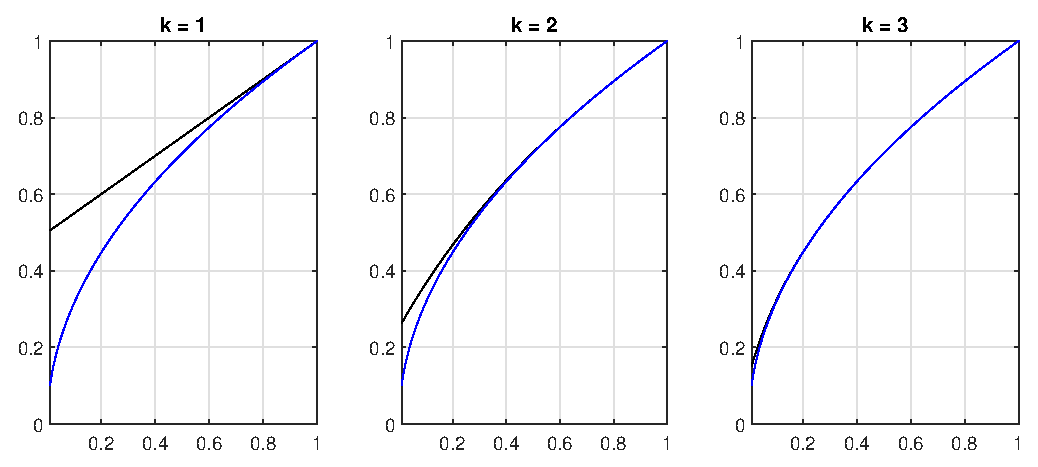
\includegraphics[width=\textwidth,height=\textheight,keepaspectratio]{figures/chapter_2/Newton_overshoot.eps}
   \caption{Newton iterates $f_{k+1}(x)=(f_k(x)+x/f_k(x))/2$ (black), plotted with $\sqrt{x}$ (blue) on $[\delta^2,1]$, where $\delta=0.1$. The $f_k$ always overestimate $f$ in the sense of \eqref{overest}.}
   \label{fig:overshootnewton}
\end{figure}

Figure \ref{fig:overshootnewton} demonstrates this effect, which is problematic because it means that the error in iterations can never equioscillate, for instance. With the aim of finding a sequence that satisfies $s'_ks''_k=1$, Ninomiya proposes the improved Newton iterates
\begin{align}
   F_{k+1}(x) = \dfrac{C_{k+1}}{2}\left(F_k(x)+\dfrac{x}{F_k(x)}\right), \qquad k=0,1,2,\dots, \label{improvnewty}
\end{align}
with $F_0=f_0/\sqrt{s'_0s''_0}$. The constants $C_{k+1}$ are given by
\[C_{k+1} = \dfrac{1}{\sqrt{N^*(S''_{k})}}, \qquad S''_k = \max_{x\in I} \dfrac{F_k(x)}{\sqrt{x}}.\]

\begin{figure}[t!]
\centering
   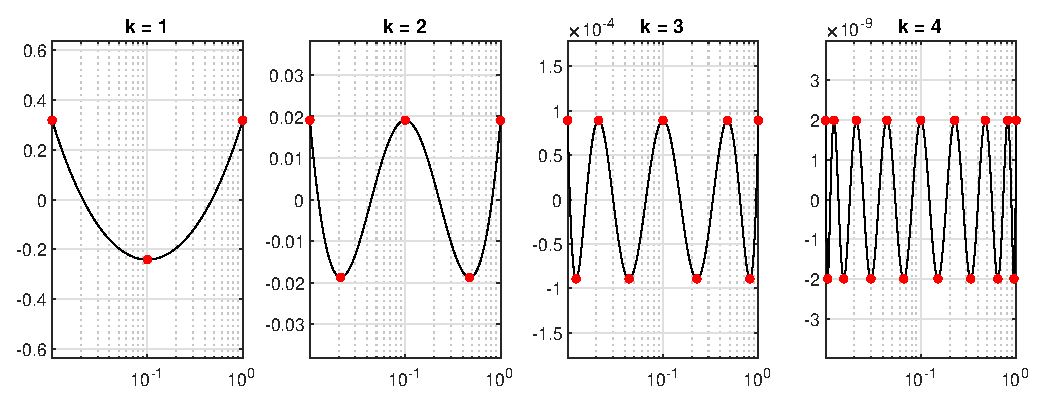
\includegraphics[width=\textwidth,height=\textheight,keepaspectratio]{figures/chapter_2/improvednewton_rational.eps}
    \caption{Relative error $E_k(x)=F_k(x)/\sqrt{x}-1$ in Ninomiya's improved Newton iterates \eqref{improvnewty} to $\sqrt{x}$ on $[\delta^2,1]$, where $\delta=0.1$.}
   \label{fig:improvednewton_rational}
\end{figure}

Assuming that we have optimised our initial guess so that $s'_0s''_0=1$, Ninomiya analyses the convergence of the $F_k$ using the following recursions, whose proofs were omitted from his paper. We prove them here as a technical lemma.

\begin{lemma}\label{EEEk}
The maximum relative errors $e''_k=s''_k-1$ and $E''_k=S''_k-1$ satisfy
\[e''_{k+1}=\dfrac{{e''_k}^2}{2(1+e''_k)}, \qquad E''_{k+1}=\sqrt{\dfrac{{E''_k}^2}{2(1+E''_k)}+1}-1.\]
\end{lemma}

\begin{proof}
Let $e_k(x)=s_k(x)-1$ and $E_k(x)=S_k(x)-1$ be the relative errors of $f_k(x)$, $F_k(x)$ respectively. Then
\begin{align*}
    e_{k+1}(x) &= s_{k+1}(x)-1 \\
    & = \dfrac{1}{2}\left(s_k(x)+\dfrac{1}{s_k(x)}\right) -1\\
    & = \dfrac{1}{2}\left(e_k(x)+1+\dfrac{1}{e_k(x)+1}\right) -1\\
    &=\dfrac{e_k(x)^2}{2(1+e_k(x))}.
\end{align*}
Since $x \mapsto x^2(1+x)^{-1}$ is an increasing function on $[0,1]$, $e_{k+1}(x)$ obtains its maximum when $e_k(x)$ is maximised, i.e. $e''_{k+1}={e''_k}^2/(2(1+e''_k))$. Similarly we have
\begin{align*}
    E_{k+1}(x) & =S_{k+1}-1 \\
    &=\dfrac{C_{k+1}}{2}\left(S_k(x)+\dfrac{1}{S_k(x)}\right) -1 \\
    &=\dfrac{1}{2\sqrt{N^*(E''_k+1)}}\left(E_k(x)+1+\dfrac{1}{E_k(x)+1}\right) -1 \\
    &=\dfrac{1}{\sqrt{N^*(E''_k+1)}}\left(\dfrac{E_k(x)^2}{2(1+E_k(x))}+1\right)-1.
\end{align*}
As before, $E_{k+1}(x)$ obtains its maximum when $E_k(x)$ is maximised, giving
\begin{align*}
    E''_{k+1}&=\dfrac{1}{\sqrt{N^*(E''_k+1)}}\left(\dfrac{{E''_k}^2}{2(1+E''_k)}+1\right)-1 \\
    &= \sqrt{\dfrac{{E''_k}^2}{2(1+E''_k)}+1}-1,
\end{align*}
by definition of $N^*$, as required.
\end{proof}

By Lemma \ref{EEEk} and a Taylor expansion, we obtain the approximate relations
\[e''_{k+1} \sim \dfrac{{e''_k}^2}{2}, \qquad E''_{k+1} \sim \dfrac{{E''_k}^2}{4}\]
as $k\to\infty$. Combining with $E''_0=e''_0$, we obtain the approximate relation
\[E''_k \sim \dfrac{e''_k}{2^{2^k-1}},\]
demonstrating that the iterates \eqref{improvnewty} improve convergence. Figure \ref{fig:improvednewton_rational} sketches the relative error of the improved Newton iterates \eqref{improvnewty}, which appear to be the best rational approximants in the relative sense as they have the correct number of equioscillation points\footnote{To see this, we note that $F_k$ is of type $(2^{k-1},2^{k-1}-1)$ by induction, hence the best rational approximant equioscillates between at least $2^k+1-d_{F_k}$ extrema by Theorem \ref{equithmrats}.}. However, they do not equioscillate between $\pm E''_k$ upon closer inspection. Ninomiya shows that the $F_k$ are best approximations over all $R$ of the same order with respect to the error of $g(x,R(x))$ relative to $\sqrt{x}$, where $g$ is the standard Newton iteration \eqref{iter} for $\sqrt{x}$ (see \cite[Theorem 4]{ninomiya1970best} for details). 

\bigskip{}

While Ninomiya's improved Newton iteration \eqref{improvnewty} is not a composite polynomial approximation to $\sqrt{x}$, we can consider his work as motivation for constructing such an approximation. Ideally, the error of our approximation should not display an upward bias, and have a similar error curve to that of Figure \ref{fig:improvednewton_rational}. In general, this dissertation is concerned with constructing polynomial approximations, such as to the Newton-Schulz approximation \eqref{scalarNSsign} to $\sgn(x)$ and the Alternative Newton approximation \eqref{altnewt} to $\sqrt{x}$, for which the convergence is accelerated. From the discussion of this section, it seems reasonable that suitably scaling the existing methods at each iteration is a sure-fire way to proceed. In the next chapter, we take a different approach to constructing an approximation to the sign function, yet discover that our method is in fact equivalent to a scaled Newton-Schulz method.

%\subsection{Halley's Method}

%An advance on Newton's Method for rootfinding is due to Halley, who developed an algorithm which finds approximations to $C^2$ functions with a cubic convergence rate. The derivation is as follows: consider a function $f$ with unknown root $x^*$, and its second-order Taylor approximation
%\[f(x) \approx f(x_k) + f'(x_k)(x-x_k) + \dfrac{f''(x_k)}{2}(x-x_k)^2,\]
%where $x_k$ is an approximate root of $f$. In a similar way to Newton's Method, we use the Taylor approximation to determine a point $x_{k+1}$ that better approximates $x^*$ than $x_k$. For this we solve
%\[f(x_k) + f'(x_k)(x_{k+1}-x_k) + \dfrac{f''(x_k)}{2}(x_{k+1}-x_k)^2 = 0,\]
%which can be factorised and re-arranged to obtain
%\[x_{k+1}-x_k= \dfrac{-f(x_k)}{f'(x_k)+\frac{f''(x_k)}{2}(x_{k+1}-x_k)}.\]
%By replacing $x_{k+1}-x_k$ on the right hand side with the error between consecutive iterates in Newton's Method, i.e. $x_{k+1}-x_k = -f(x_k)/f'(x_k)$, we obtain
%\begin{align}
%    x_{k+1} = x_k -\dfrac{2f(x_k)f'(x_k)}{2f'(x_k)^2-f(x_k)f''(x_k)}.\label{halley}
%\end{align}
%The iterative procedure \eqref{halley} is known as Halley's Method.

%\bigskip{}

%\begin{ex}
%Suppose for some $\lambda >0$ we want to approximate the value of $1/\sqrt{\lambda}$. This is equivalent to finding the positive root of $f(x)=1/x^2 -\lambda=0$. Then \eqref{halley} reads
%\begin{align}
%    x_{k+1} = \dfrac{x_k}{8}\left(15-\lambda x_k^2(10-3\lambda x_k^2)\right).\label{halleyrecip}
%\end{align}
%\end{ex}



%\newpage
%\thispagestyle{empty}
%\mbox{}